%\setcounter{section}{-1}% set to Kapitel 0 % Macht Probleme, wenn zuvor schon \section{...} aufgerufen wurde z.B. bei Zusammenfügen von mehreren Modulen

\section{Wiederholung}
%\begin{frame}\ftx{\secname}
% Kapitel 1
\s{% Skript-only
    Um das frequenz- und zeitabhängige Verhalten elektrischer Netzwerke zu beschreiben, 
    werden in diesem Kapitel kurz einige wichtige Grundlagen zusammengefasst. 

    Zur Bearbeitung vorrausgesetzt werden Kenntnisse über elektrische Grundgrößen, 
    lineare passive Bauteile $R$, $L$ und $C$, Netzwerkberechnungen, 
    sowie die komplexe Wechselstromrechnung.
}
%\end{frame}

%%%%%%%%%%%%%%%%%%%%%%%%%%%%%%%%%%%%%%%%%%%%%%%%%%%%%%%%%%%%%%%%%%%%%%%%%%%%%%%%%%%%%

\subsection{Frequenzabhängigkeit elektrischer Bauelemente}
\begin{frame}\ftx{\subsecname}
\s{% Skript-only
    Rein ohmsche Widerstände $R$ können elektrische keine Energie speichern. 
    Spannungen und Ströme sind proportional zueinander und zu jedem Zeitpunkt in Phase.
    Das Verhalten ist zeit- und frequenzunabhängig.

    Induktivitäten $L$ und Kapazitäten $C$ hingegen können Energie speichern und abgeben.
    Dieser Vorgang ist inert (träge), benötigt also eine gewisse Zeit. 
    Dadurch verhalten sie sich frequenzabhängig. 

    Ströme und Spannungen stehen bei Induktivitäten und Kapazititäten in (zeitlich) differentiellem 
    linearen Verhältnis zueinander. Dadurch entsteht bei beiden Bauteiltypen eine Phasenverschiebung 
    zwischen Spannung und Strom von betragsmäßig $90\ \degree$.

    Abbildung \ref{fig:bauteile:phasenverschiebung} zeigt die Spannungs- und Stromverläufe für $R$, $L$ und $C$
    bei Erregung mit einer Wechselspannung $u_q = U \cdot \sin(\omega t)$ zum Vergleich.

    \begin{figure}[H]\centering
        \begin{subfigure}{0.68\textwidth}\centering
            \includegraphics{Tikz/pdf/plot_bauteile_phasenverschiebung_r.pdf}
        \end{subfigure}%
        \begin{subfigure}{0.28\textwidth}\centering
            \includegraphics{Tikz/pdf/circ_bauteil_R_u_i.pdf}% R
        \end{subfigure}\hfill% newline
        \begin{subfigure}{0.68\textwidth}\centering
            \includegraphics{Tikz/pdf/plot_bauteile_phasenverschiebung_l.pdf}
        \end{subfigure}%
        \begin{subfigure}{0.28\textwidth}\centering
            \includegraphics{Tikz/pdf/circ_bauteil_L_u_i.pdf}% L
        \end{subfigure}\hfill% newline
        \begin{subfigure}{0.68\textwidth}\centering
            \includegraphics{Tikz/pdf/plot_bauteile_phasenverschiebung_c.pdf}
            \caption{Strom- und Spannungsverläufe}
        \end{subfigure}%
        \begin{subfigure}{0.28\textwidth}\centering
            \includegraphics{Tikz/pdf/circ_bauteil_C_u_i.pdf}% C
            \caption{Schaltsymbole}
        \end{subfigure}
        \caption{Phasenverschiebung bei $R$, $L$ und $C$}\label{fig:bauteile:phasenverschiebung}
    \end{figure}

    Aufgrund der Phasenverschiebung bei $L$ und $C$ oszilliert deren Leistung 
    (Energieaufnahme und -abgabe), ist über eine Periode gemittelt jedoch immer null.
    Induktivitäten und Kapazitäten können daher keine Wirkleistung, sondern nur Blindleistung
    verrichten, weshalb sie auch Blindwiderstände genannt werden.
}
\b{% Folien-only
    %3 AC Plots: u(t), i(t) mit $\varphi$ eingezeichnet für $R$, $L$, $C$
    \begin{minipage}{\textwidth}\centering
        \onslide<1->{%
        \begin{minipage}{0.68\textwidth}\centering
            \resizebox{0.7\textwidth}{!}{\includegraphics{Tikz/pdf/plot_bauteile_phasenverschiebung_r.pdf}}   % plot \onslide<1->{...}        <-- OVERLAY
        \end{minipage}%
        }%
        \begin{minipage}{0.28\textwidth}\centering
            \includegraphics{Tikz/pdf/circ_bauteil_R_u_i.pdf}% R
        \end{minipage}\hfill% newline
        \onslide<2->{%
        \begin{minipage}{0.68\textwidth}\centering
            \resizebox{0.7\textwidth}{!}{\includegraphics{Tikz/pdf/plot_bauteile_phasenverschiebung_l.pdf}}   % plot \onslide<2->{...}        <-- OVERLAY
        \end{minipage}%
        }%
        \begin{minipage}{0.28\textwidth}\centering
            \includegraphics{Tikz/pdf/circ_bauteil_L_u_i.pdf}% L
        \end{minipage}\hfill% newline
        \onslide<3->{%
        \begin{minipage}{0.68\textwidth}\centering
            \resizebox{0.7\textwidth}{!}{\includegraphics{Tikz/pdf/plot_bauteile_phasenverschiebung_c.pdf}}   % plot \onslide<3->{...}        <-- OVERLAY
        \end{minipage}%
        }%
        \begin{minipage}{0.28\textwidth}\centering
            \includegraphics{Tikz/pdf/circ_bauteil_C_u_i.pdf}% C
        \end{minipage}
    \end{minipage}
    \speech{folie1}{1}{Dies ist ein Beispiel Text. A + i mal B gleich C komplex. Hundert Volt Spannung.}
}% end Folien-only
\end{frame}

%%%%%%%%%%%%%%%%%%%%%%%%%%%%%%%%%%%%%%%%%%%%%%%%%%%%%%%%%%%%%%%%%%%%%%%%%%%%%%%%%%%%%

\subsubsection{Verhalten von Induktivitäten und Kapazitäten}
\begin{frame}\ftx{\subsubsecname}
\s{% Skript-only
    Induktivitäten als ideale Bauteile speichern durch den Effekt der (Selbst-)Induktion Energie im Magnetfeld.
    Kapazitäten als ideale Bauteile hingegen speichern Energie im elektrischen Feld. 
    Beschrieben werden beide Effekte durch das Induktion- beziehungsweise das Gaußsche Gesetz.

    Tabelle \ref{tab:vergleich:induktivitaetkapazitaet} listet die wichtigsten Unterschiede 
    im Verhalten von Induktivitäten und Kapazitäten qulitativ als Übersicht auf.

    \begin{table*}[h]\centering
    \caption{Vergleich von Induktivität und Kapazität im Verhalten}
    \label{tab:vergleich:induktivitaetkapazitaet}
    \begin{tabular}{ccc}
        \toprule&\textbf{Induktivität} &\textbf{Kapazität}\\
        \midrule
        \textbf{Gesetz}         &Induktionsgesetz       &Gaußsches Gesetz   \vphantom{$\Big|$}\\
        \textbf{Energiespeich.} &im Magnetfeld          &im Elektr. Feld    \vphantom{$\Big|$}\\
        \textbf{stetig}         &Strom                  &Spannung           \vphantom{$\Big|$}\\
        \textbf{bei Gleichspg.} &Kurzschluss            &offen              \vphantom{$\Big|$}\\
        \textbf{bei Hochfreq.}  &offen                  &Kurzschluss        \vphantom{$\Big|$}\\
        \bottomrule
    \end{tabular}
    \end{table*}

    Die (Selbst-)Induktivität $L$ als Eigenschaft kann vereinfacht als \glqq Trägheit \grqq des Stroms
    betrachtet werden. Ströme in Induktivitäten sind stetig und eilen der Spannung hinterher.
    Bei hohen Frequenzen sperrt die Induktivität, bei Gleichspannung verhält sie sich wie ein Kurzschluss.
    
    Die Kapazität $C$ kann dem gegenüber vereinfacht als \glqq Trägheit \grqq der Spannung betrachtet werden.
    Spannungen in Kapazitäten sind stetig und eilen dem Strom hinterher. 
    Bei Gleichstrom sperrt die Kapazität, bei hohen Frequenzen verhält sie sich wie ein Kurzschluss.

    \begin{figure}[H]\centering
        \begin{subfigure}{0.45\textwidth}\centering
            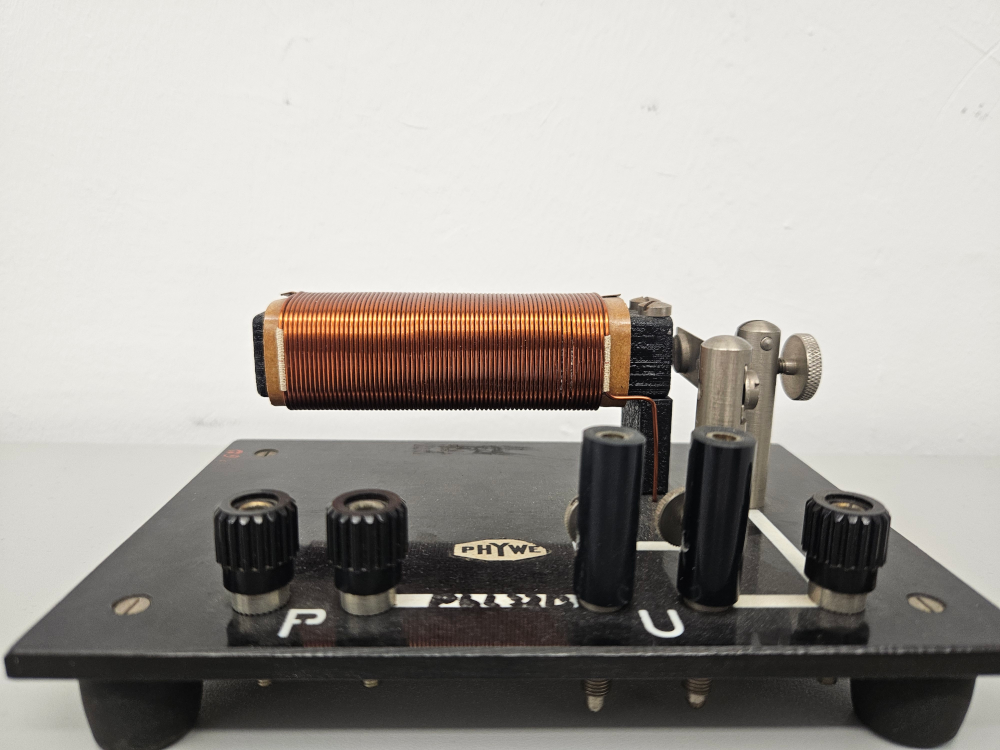
\includegraphics[width=0.75\textwidth]{./Bilder/Spule.png}
        \end{subfigure}%
        \begin{subfigure}{0.45\textwidth}\centering
            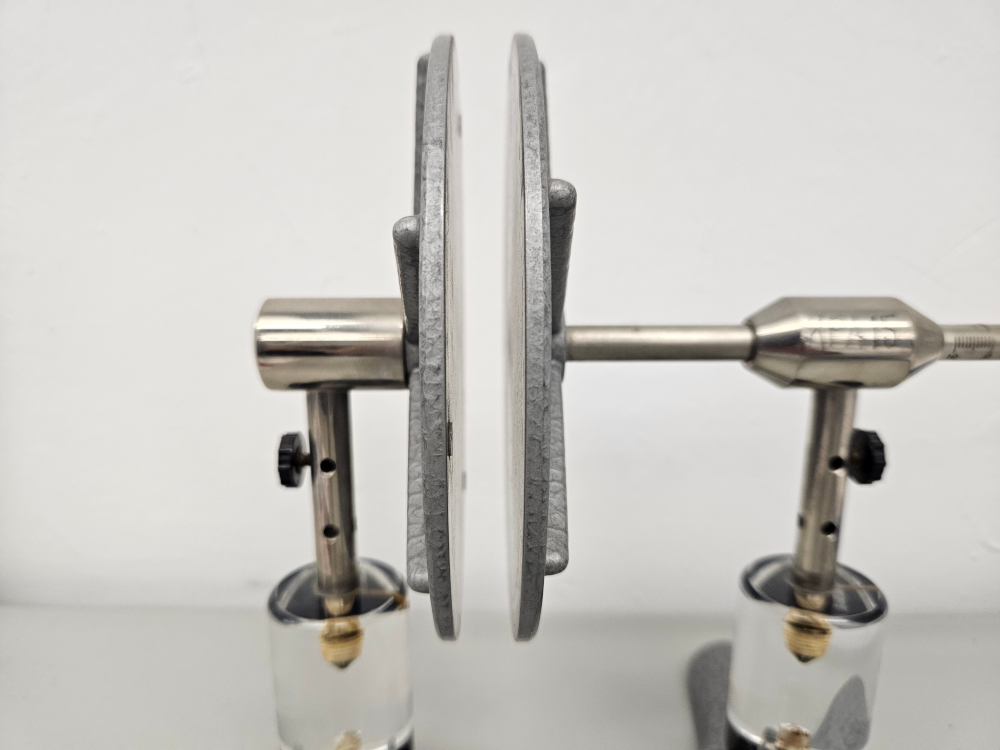
\includegraphics[width=0.75\textwidth]{./Bilder/Kondensator.png}
        \end{subfigure}
        \caption{Reale Induktivät (Spule, links) und Kapazitäten (Kondensator, rechts)}\label{fig:bauteile:realebauteile}
    \end{figure}
    Abbildung \ref{fig:bauteile:realebauteile} zeigt reale Bauteile, die Induktivitäten und Kapazitäten realisieren. 
    Gezeigt sind eine Spule (Induktivität) und ein Kondensator (Kapazität).
}
\b{% Folien-only
\begin{columns}
\column{0.35\textwidth}
    \textbf{Induktivität}%
    \begin{itemize}
        \item Impedanz: $\underline{Z}_{\mathrm L} = \mathrm{j}\omega L$
        \item DGL: $\ecv{u_{\mathrm L}} = L \cdot \frac{\d}{\d t}\, \eci{i_{\mathrm L}}$
        \item Energie im Magnetfeld
        \item Ströme stetig (keine Sprünge)
    \end{itemize}

    \textbf{Kapazität}%
    \begin{itemize}
        \item Impedanz: $\underline{Z}_{\mathrm C} = -\mathrm{j}\frac{1}{\omega C}$
        \item DGL: $\eci{i_{\mathrm C}} = C \cdot \frac{\d}{\d t}\, \ecv{u_{\mathrm C}}$
        \item Energie im elektrischen Feld
        \item Spannungen stetig (keine Sprünge)
    \end{itemize}

\column{0.15\textwidth}\centering
    \includegraphics{Tikz/pdf/circ_bauteil_L_u_i_mini.pdf}% Schaltsymbol
    \vspace{2cm}
    \includegraphics{Tikz/pdf/circ_bauteil_C_u_i_mini.pdf}% Schaltsymbol

\column{0.5\textwidth}
    \begin{figure}[H]\centering
        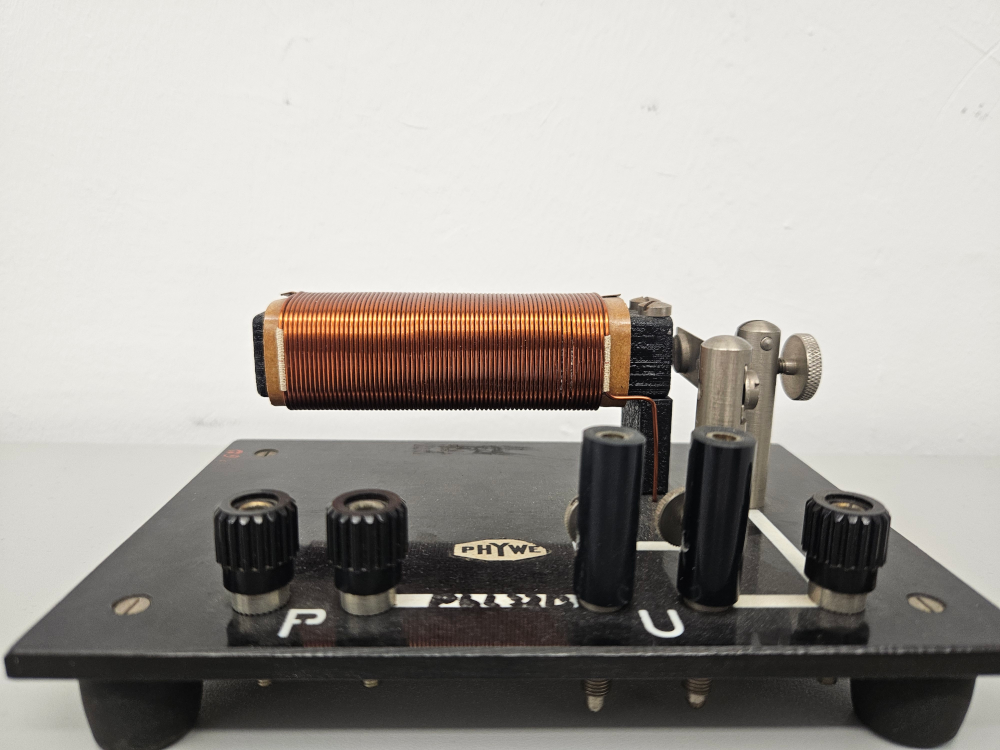
\includegraphics[width=0.5\textwidth]{./Bilder/Spule.png}
        \par Spule
    \end{figure}
    \begin{figure}\centering
        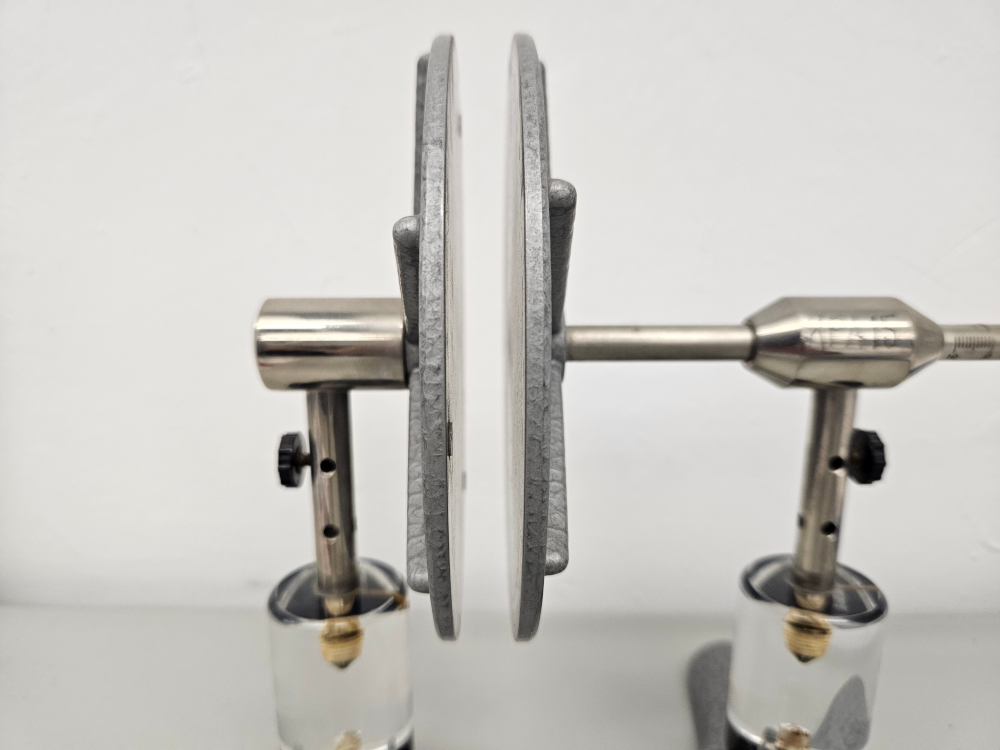
\includegraphics[width=0.5\textwidth]{./Bilder/Kondensator.png}
        %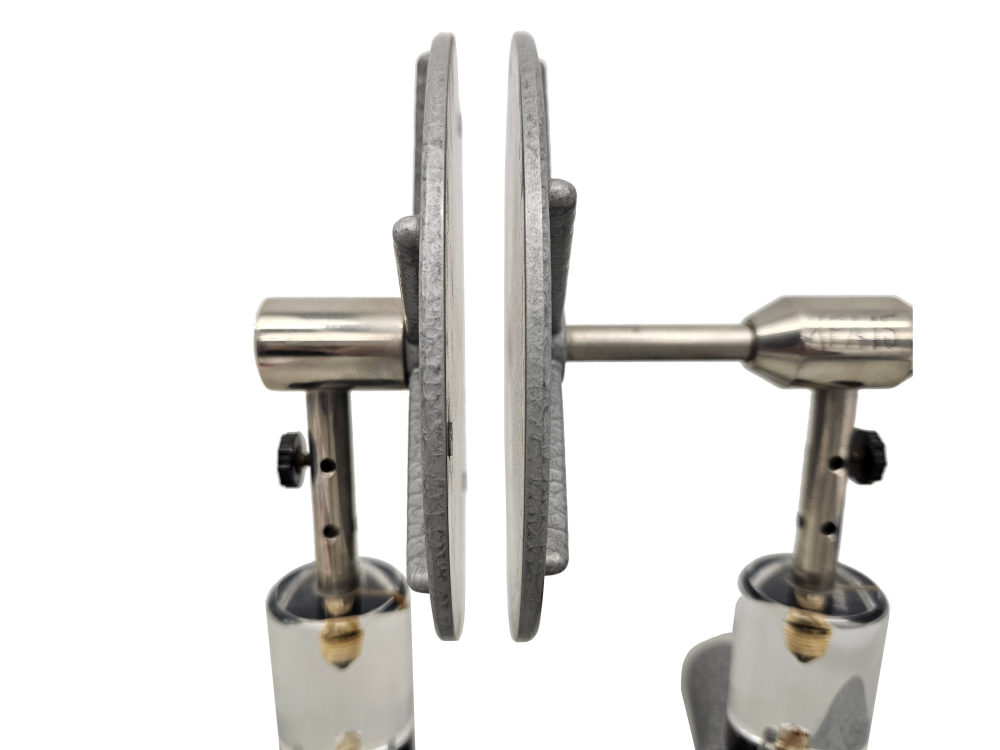
\includegraphics[width=0.5\textwidth]{./Bilder/Kondensator_cut.png}
        \par Kondensator
    \end{figure}
\end{columns}
}% end Folien-only
\end{frame}

%%%%%%%%%%%%%%%%%%%%%%%%%%%%%%%%%%%%%%%%%%%%%%%%%%%%%%%%%%%%%%%%%%%%%%%%%%%%%%%%%%%%%

\subsubsection{Vergleich der linearen Zweipole $R$, $L$ und $C$}
\begin{frame}\ftx{\subsubsecname}

    \s{\ref{tab:vgl:bauteile:rlc} zeigt eine Gegenüberstellung der Größen $R$, $L$ und $C$ und fasst deren wichtigsten Eigenschaften zusammen. }

    \begin{table}[h]\centering%
    \s{\caption{Vergleich lineare Bauteile $R$, $L$, $C$}\label{tab:vgl:bauteile:rlc}}%
    \resizebox{\textwidth}{!}{% for beamer page fit
    \begin{tabular}{ |c|c|c|c|c| }
        \hline &&&&\\[-6pt]
        \textbf{Größe}                          % Col 1
                & \textbf{Allgemein}            % Col 2
                & \textbf{El. Widerstand}       % Col 3
                & \textbf{Induktivität}         % Col 4
                & \textbf{Kapazität} \\[+4pt]   % Col 5
        \hline%
        %\textbf{Symbol}
        \includegraphics{Tikz/pdf/circ_bauteil_tabelle_text_symbol.pdf}% Symbol (vertikal zentriert)
                & \includegraphics{Tikz/pdf/circ_bauteil_tabelle_zweipol.pdf}
                & \includegraphics{Tikz/pdf/circ_bauteil_tabelle_R.pdf}
                & \includegraphics{Tikz/pdf/circ_bauteil_tabelle_L.pdf}
                & \includegraphics{Tikz/pdf/circ_bauteil_tabelle_C.pdf} \\[+4pt]
        \hline &&&&\\[-6pt]
        %\textbf{Bauteil}
        %        & Zweipol
        %        & Widerstand
        %        & Spule
        %        & Kondensator \\[+4pt]
        %\hline &&&&\\[-6pt]
        \textbf{Einheit}
                & $ \left[\textit{Form.z.}\right] = \mathrm{Einheit} $ 
                & $ \left[R\right] = \Omega\ \text{(Ohm)} $     
                & $ \left[L\right] = \mathrm{H}\ \text{(Henry)} $ 
                & $ \left[C\right] = \mathrm{F}\ \text{(Farad)} $ \\[+4pt]
        \hline &&&&\\[-6pt]
        \textbf{Zeitbereich}
                & $ \frac{\d}{\d t} $ bzw. $ \int \d t $ 
                & $ \ecv{u_{\mathrm{R}}} = R \cdot \eci{i_{\mathrm R}} $     
                & $ \ecv{u_{\mathrm{L}}} = L \cdot \frac{\d}{\d t}\, \eci{i_{\mathrm{L}}} $ 
                & $ \eci{i_{\mathrm{C}}} = C \cdot \frac{\d}{\d t}\, \ecv{u_{\mathrm{C}}} $ \\[+4pt]
        \hline &&&&\\[-6pt]
        \textbf{Frequenzb.}
                & $ \mathrm{j}\omega $ bzw. $ \frac{1}{\mathrm{j}\omega} $
                & $ \ecv{\underline{U}_{\mathrm R}} = R                   \cdot \eci{\underline{I}_{\mathrm R}} $ 
                & $ \ecv{\underline{U}_{\mathrm L}} = \mathrm{j}\omega L  \cdot \eci{\underline{I}_{\mathrm L}} $
                & $ \eci{\underline{I}_{\mathrm C}} = \mathrm{j}\omega C  \cdot \ecv{\underline{U}_{\mathrm C}} $ \\[+4pt]
        \hline &&&&\\[-6pt]
        \textbf{Impedanz}
                & $ \underline{Z} = \frac{\ecv{\underline{U}}}{\eci{\underline{I}}} $
                & $ \underline{Z}_{\mathrm R} = R $ 
                & $ \underline{Z}_{\mathrm L} = \mathrm{j}\omega L $
                & $ \underline{Z}_{\mathrm C} = -\mathrm{j}\frac{1}{\omega C} $ \\[+4pt]
        \hline &&&&\\[-6pt]
        \textbf{Wirkanteil}
                & $ R = \Re\{\underline{Z}\} $
                & $ R = \frac{U}{I} $
                & $ 0 $
                & $ 0 $ \\[+4pt]
                \hline &&&&\\[-6pt]
        \textbf{Blindanteil}
                & $ X = \Im\{\underline{Z}\} $
                & $ 0 $
                & $ X_{\mathrm L} = \omega L $
                & $ X_{\mathrm C} = -\frac{1}{\omega C}$ \\[+4pt]
        \hline
    \end{tabular}
    } % end resizebox
    \end{table}
    
% Für Schaltungen variabler Frequenz: Frequenzvariablen Eigenschaften von Bauteilen, dafür zeitvariante 
\end{frame}

%%%%%%%%%%%%%%%%%%%%%%%%%%%%%%%%%%%%%%%%%%%%%%%%%%%%%%%%%%%%%%%%%%%%%%%%%%%%%%%%%%%

% Beschreibe in Textform wie das Verhalten von Eingangs- zu Ausgangssignalen eines Vierpols 
% mithilfe des Frequenzgangs (bzw. des Amplituden- und Phasengangs) beschrieben werden kann
\s{
\subsection{Zweitore (Vierpole)}
\begin{frame}\ftx{\subsecname}


    % Wiederholung Eintor
    Die Frequenzabhängigkeit von Eintoren (Zweipole) haben wir in Modul 3 bereits untersucht.  
    Mithilfe der komplexen Wechselstromrechnung konnten wir den frequenzabhängigen Wechselstromwiderstand 
    (Impedanz) $\underline{Z}$ einzelner Eintore bestimmen. Durch Anwendung der komplexen Strom- 
    und Spannungsteilerregel konnten wir auch die Gesamt-Impedanz linearer zweipoliger Netzwerke bestimmen. 
    Das heißt für solche, welche nur aus linearen Bauteilen wie $R$, $L$ und $C$ bestehen. 

    % Tikzpicture: Vergleich Vierpol und Zweipol
    %
    % Zeichne links einen senkrechten Zweipol mit Spannungs- (U) und Strompfeil (I) jeweils von oben nach unten
    % Zeichne rechts einen Vierpol (Eingangspole links, Ausgangspole rechts) (U1 links oben nach unten, U2 rechts oben nach unten)
    \begin{figure}[h]
        \begin{subfigure}{0.48\textwidth}\centering
            \includegraphics{Tikz/pdf/circ_eintor.pdf}
        \end{subfigure}\hfill
        \begin{subfigure}{0.48\textwidth}\centering
            \includegraphics{Tikz/pdf/circ_zweitor.pdf}
        \end{subfigure}
        \caption{Vergleich: Schaltzeichen eines allgemeinen Zwei- und Vierpols}
        \label{fig:vgl:zweipolvierpol}
    \end{figure}

    % Einführung Zweitor, wozu
    Zweitore (Vierpole) sind eine Erweiterung von Eintoren (Zweipolen).
    Sie verfügen über eine Eingangs- und eine Ausgangsseite mit jeweiligen Eingangs- und Ausgangsgrößen.  
    Das Zweitormodell eignet sich gut zur Beschreibung von (frequenzabhängigen) Übertragungseigenschaften 
    von elektrischen Netzwerken. 

    \fu{\includegraphics{Tikz/pdf/circ_zweitor_quelle_last.pdf}
    }{Verbindung einer Last über ein Zweitor mit der Quelle.\label{circ:quellezweitorlast}}% im Foliensatz im nächsten Kapitel (Freuqenzgang, Amplitudengang, Phasengang)
    
    Im einfachsten Fall wird wie in \ref{circ:quellezweitorlast} gezeigt, eine Quelle (Eintor) über ein Zweitor 
    mit einer Last (Eintor) verbunden. 
    Typische Zweitore sind beispielsweise Verstärker, Filter oder auch Transformatoren. 
\end{frame}
}% end skript only


